% !TeX TS-program = pdflatex
% !TeX encoding = UTF-8
% !TeX spellcheck = it_IT
% !TeX root = MyThesis.tex

\documentclass[12pt,a4paper,twoside,openright,fleqn,titlepage]{report}
% default: 10pt -> 12pt
% default: letterpaper -> a4paper
% default: oneside -> twoside
% default: openany -> openright
% default: titlepage
% default: final
% added: fleqn
% -------------------------------- %
% general packages
% -------------------------------- %
\usepackage[T1]{fontenc}
\usepackage{textcomp} % scelta dei font
\usepackage[utf8]{inputenc} % encoding
\usepackage[english,italian]{babel}
\hyphenation{} % hyphen specialized terms
\usepackage{microtype}
\usepackage{indentfirst}
\usepackage[heightrounded,bindingoffset=5mm]{geometry}
\usepackage{lipsum} % dummy text
% -------------------------------- %
% bibliography
% -------------------------------- %
\usepackage[autostyle,italian=guillemets,babel]{csquotes}
\usepackage[backend=biber,useprefix,style=ieee,backref,hyperref,defernumbers=true]{biblatex} % IEEE style
%\usepackage[authordate,autocite=inline,backend=biber,natbib,backref,hyperref=true]{biblatex-chicago} % Chicago style
\addbibresource{MyThesisBib.bib}
% -------------------------------- %
% maths and numbers
% -------------------------------- %
\usepackage{siunitx}
\sisetup{%
	output-decimal-marker={,}, group-separator={\,},%
	round-mode=places%
}
% -------------------------------- %
% floating objects
% -------------------------------- %
\usepackage{graphicx}
\usepackage{tabularx}
\usepackage{booktabs}
\usepackage{multirow}
\usepackage{longtable}
\usepackage{flafter}
%\usepackage{placeins} % \FloatBarrier
% -------------------------------- %
% other packages
% -------------------------------- %
\usepackage[strict]{changepage}
\usepackage{relsize} % relsize{}
\usepackage{pdfpages}
\usepackage{enumitem}
\usepackage[italian,nospace]{varioref} % \vref{}
\usepackage[bottom]{footmisc}
\interfootnotelinepenalty=10000
\dimen\footins=2.5cm
\usepackage{xspace}
% -------------------------------- %
% dnthesis
% -------------------------------- %
% compacttoc (move page number near toc entry)
% arscaptions (figure, table and code captions)
% arscolors (hyperref colors)
% contnum (continuous floating objects numbering)
% printing (when it's time to send to the printer)
\usepackage[arscaptions,arscolors,contnum]{dnthesis}

% code settings

\definecolor{lightergray}{gray}{0.99}

\addto\captionsitalian{%
	\renewcommand{\lstlistingname}{Codice}
	\renewcommand{\lstlistlistingname}{Elenco dei codici}}

% -------------------------------------------------------- %
% MATLAB
%\lstdefinestyle{MATLAB}{language=Matlab,
%	keywordstyle=\color{blue},
%	basicstyle=\normalfont\ttfamily,
%	commentstyle=\color{green}\ttfamily,
%	stringstyle=\rmfamily,
%	numbers=left,
%	numberstyle=\scriptsize,
%	stepnumber=1,
%	numbersep=8pt,
%	showstringspaces=false,
%	breaklines=true,
%	frameround=ftff,
%	frame=lines,
%	backgroundcolor=\color{lightergray}
%}

\lstdefinestyle{base}{%
	keywordstyle=\color{black}\bfseries,
	basicstyle=\relsize{-1.75}\ttfamily,
	backgroundcolor=\color{lightergray},
	breaklines=true,
	frameround=ftff,
	frame=lines,
	morekeywords={TITLE,ABS,KEY,AND,OR,NOT},
}

% -------------------------------------------------------- %

% -------------------------------------------------------- %
% Commands, environments and easy redefinitions
% -------------------------------------------------------- %
% Your info
\newcommand{\myTitle}{Titolo in italiano}
\newcommand{\myEngTitle}{English title}
\newcommand{\mySubject}{Thesis type}
\newcommand{\myName}{Nome Cognome}
\newcommand{\myRelatore}{Nome Cognome}
% Miscellaneous
\newcommand{\omissis}{[\textellipsis\unkern]}
\newcommand{\eng}[1]{\foreignlanguage{english}{#1}\xspace}
\newcommand{\engemph}[1]{\eng{\emph{#1}}}
\newcommand{\SLR}{\engemph{Systematic Literature Review}}
\newcommand{\slr}{\engemph{systematic literature review}}
% -------------------------------------------------------- %
%\usepackage{showframe} % show page frame
%\usepackage[reals,italian]{layout} % print the page layout, activate the command

\hypersetup{%
	pdftitle={\myTitle},%
	pdfauthor={\myName},%
	pdfsubject={\mySubject},%
	pdfkeywords={}%
}
\begin{document}
%\layout % first, activate the package
\frenchspacing
% ************************************************************************************* %
% ************************************************************************************* %
% FRONTMATTER
% ************************************************************************************* %
% ************************************************************************************* %
\pagenumbering{roman}\pagestyle{empty}
% dedication + abstract

% --------------------------------------------------------- %
% DEDICA
% --------------------------------------------------------- %
\pdfbookmark{Dedica}{edication}

\begin{flushright}
{\em \lipsum[1][1-2]}
\end{flushright}\cleardoublepage
% --------------------------------------------------------- %
% SOMMARIO
% --------------------------------------------------------- %
\pdfbookmark{Sommario}{sommario}

\begin{abstract}
\lipsum[1]\par\smallskip\lipsum[2]\par\smallskip\lipsum[3]
\end{abstract}
\cleardoublepage
% ------------------------------------------------------------------------------------- %
\pagenumbering{arabic}\pagestyle{main}
\pdfbookmark{\contentsname}{tableofcontents}

\setcounter{tocdepth}{1} % profondità, fino a quale livello arrivare
\tableofcontents
%\cleardoublepage
%\listoffigures
%\listoftables
%\begingroup
%\renewcommand*{\addvspace}[1]{}
%\pdfbookmark{\listfigurename}{listoffigures}
%\listoffigures\cleardoublepage
%\pdfbookmark{\listtablename}{listoftables}
%\listoftables
%\endgroup
\cleardoublepage
\pagestyle{nosec}
\pdfbookmark{Ringraziamenti}{Ringraziamenti}

\chapter*{Ringraziamenti}

\lipsum[1]
\cleardoublepage\pagestyle{main}\cleardoublepage
% ************************************************************************************* %
% ************************************************************************************* %
% MAINMATTER %
% ************************************************************************************* %
% ************************************************************************************* %
\pagestyle{nosec}% ***************************************************** %
\chapter{Introduzione}\label{ch:intro}
% ***************************************************** %

\lipsum[1]

\begin{itemize}
\item \MakeTextLowercase{\lipsum[1][1]}
\item \MakeTextLowercase{\lipsum[1][2]}
\item \MakeTextLowercase{\lipsum[1][3]}
\end{itemize}

\lipsum[2-3]\par\bigskip

\lipsum[1][1]
\begin{description}
\item[{\hyperref[ch:chap-name]{Il secondo capitolo}}] \lipsum[1][1-2]
\item[{\hyperref[ch:concl]{Il terzo capitolo}}] \lipsum[1][2-3]
\end{description}
\cleardoublepage\pagestyle{main}\cleardoublepage

% ***************************************************** %
\chapter{Titolo breve}\label{ch:chap-name}
% ***************************************************** %

\lipsum[1]

Nell'articolo di~\textcite{provaBib} \lipsum[1][1-2]

Si veda la bellissima figura~\vref{fig:lorem3}.

\begin{figure}
\centering
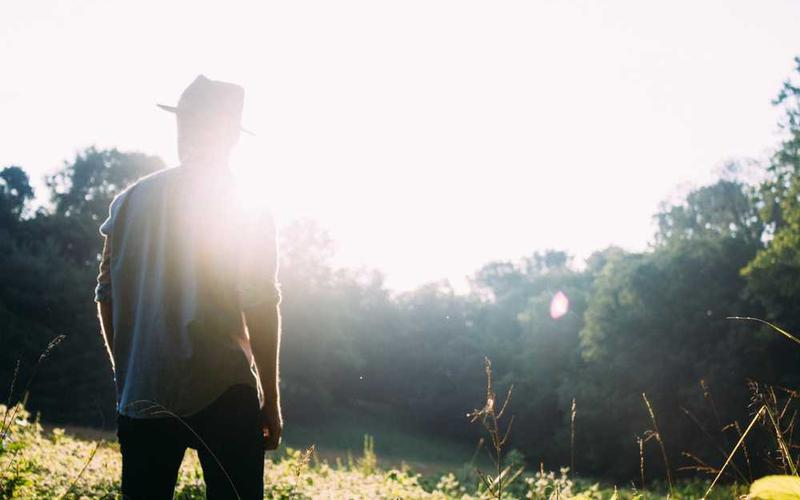
\includegraphics[width=0.4\textwidth]{./Figures/img2.jpg}
\caption{Figura completamente a caso}
\label{fig:lorem3}
\end{figure}

\section{Titolo breve del paragrafo}

\lipsum[1]

\subsection{Titolo della dimensione che preferisci}

\lipsum[2]

\lipsum[3]

Dai uno sguardo alla tabella~\vref{tab:tab1}.

\begin{table}
\centering
\caption{Una tabella per comparare cose}
\label{tab:tab1}
\begin{tabular}{lp{0.35\textwidth}p{0.35\textwidth}}
\toprule
\textbf{Pippo} & \textbf{Pluto} & \textbf{Paperino} \\
\midrule
Primo & \lipsum[1][1] & \lipsum[1][3-4] \\
Secondo & \lipsum[1][1] & \lipsum[1][3-4] \\
Terzo & \lipsum[1][1] & \lipsum[1][3-4] \\
\bottomrule
\end{tabular}
\end{table}

\section{Sempre un titolo breve}

\lipsum[3-4]

\subsection{Titolo del sottoparagrafo}

\lipsum[1]

Si veda a proposito la figura~\vref{fig:prova_fig}.

\begin{figure}
\centering
\includegraphics[page=1]{./Figures/Drawings/MyThesis-drawings}
\caption{Un esempio di \engemph{flow chart}}
\label{fig:prova_fig}
\end{figure}

\subsubsection{Titolo di un sottosotto paragrafo della dimensione che preferisci}

\lipsum[2]

\lipsum[3]

Si veda la tabella~\vref{tab:prova_tab}.

\begin{table}
\caption{Esempio di tabella con testo}
\label{tab:prova_tab}
\begin{tabularx}{\textwidth}{lX}
\toprule
\textbf{Una cosa} & \lipsum[1][1-4] \\
\textbf{Un'altra cosa} & \lipsum[2][1-4] \\
\bottomrule
\end{tabularx}
\end{table}

\subsection{Altro titolo di sottoparagrafo}

\lipsum[1]

\section{Adesso delle figure}

\lipsum[1][1-5] come si vede nella figura~\vref{fig:lorem1}.

\begin{figure}
\centering
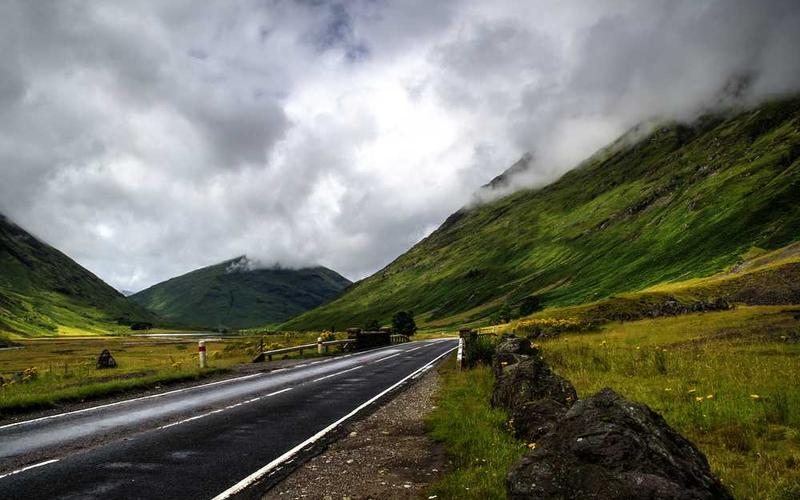
\includegraphics[width=\textwidth]{./Figures/img1.jpg}
\caption{Una figura \emph{lorem ipsum}}
\label{fig:lorem1}
\end{figure}

\lipsum[1][1-5]

\lipsum[1][1-5]

A tal proposito si vedano le figure~\ref{subfig:lorem2_1}~e~\vref{subfig:lorem2_2}.

\begin{figure}
\centering
\subfloat[][\emph{Didascalia di questa}\label{subfig:lorem2_1}]
	{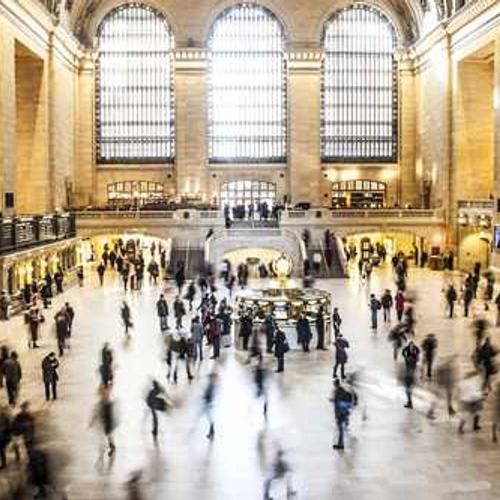
\includegraphics[width=0.45\textwidth]{./Figures/img3.jpg}} \quad
\subfloat[][\emph{Didascalia di quest'altra}\label{subfig:lorem2_2}]
	{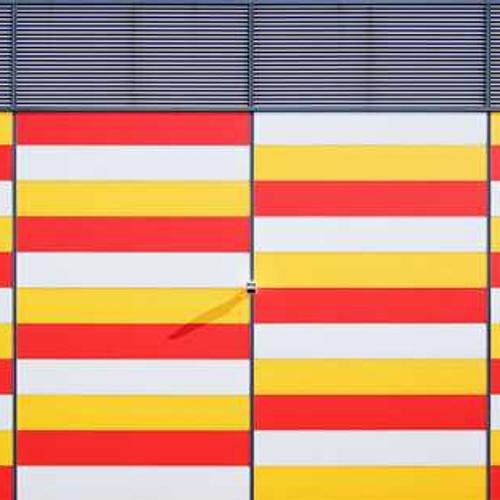
\includegraphics[width=0.45\textwidth]{./Figures/img4.jpg}}
\caption{Didascalia di un paio di figure a caso}
\label{fig:lorem2}
\end{figure}
\cleardoublepage
% ***************************************************** %
\chapter{Conclusioni e sviluppi futuri}\label{ch:concl}
% ***************************************************** %

\lipsum
\cleardoublepage
% ************************************************************************************* %
% ************************************************************************************* %
% BACKMATTER %
% ************************************************************************************* %
% ************************************************************************************* %
% biblio

% --------------------------------------------------------- %
% BIBLIOGRAFIA
% --------------------------------------------------------- %
\cleardoublepage
\pagestyle{biblio}
\phantomsection
%\chapter*{\bibname}
\inToc{\bibname}
\printbibliography
%\cleardoublepage
\end{document}
